\subsection{Изменение меры Лебега при линейных отображениях}
\begin{fact}[Из линала, б/д]
    Пусть дано обратимое л.о. $V: \R^m \rightarrow \R^m$. Тогда существуют ОНБ $\{g_j\}$ и $\{h_j\}$ и набор положительных чисел $\{c_j\}$ т.ч. \[V(x) = \sum\limits_{j = 1}^m c_j\langle x, g_j \rangle h_j\]
\end{fact}
\begin{proof}
    Рассмотрим $V^*$~---~сопряжённое к $V$ преобразование и $W = V^*V$~---~с/с преобразование. Для $W$  существует ОНБ из с.в. $\{g_j\}$, соответствующих собственным числам $\{s_j\}$. каждое такое число положительно, поскольку $\langle Wx, x \rangle = \|V(x)\|^2$ положительно определена. Пусть тогда $c_j = \sqrt{s_j}$. Тогда \[x = \sum\limits_{i = 1}^m \langle x, g_i \rangle g_i\]
    А значит \[V(x) = \sum\limits_{j = 1}^m \langle x, g_i \rangle Vg_j = \sum\limits_{j = 1}^m c_j \langle x, g_i \rangle h_j, h_j = \dfrac{1}{c_j}Vg_i\]
    Очевидно, что $\{h_j\}$~---~ОНБ.
\begin{note}
    При этом, заметим, что $|\det V| = \prod\limits_{j = 1}^m c_j$, т.к. $(\det V)^2 = \det W = \prod\limits_{j = 1}^m s_j$.
\end{note}
\end{proof}

\begin{theorem}
    Пусть дано обратимое л.о. $V: \R^m \rightarrow \R^m$ и измеримое $E$. Тогда $V(E) \in \MM^m$ и \[\LL^m(V(E)) = |\det V| \LL^m(E)\]
\end{theorem}
\begin{proof}
    В силу гладкости л.о. $\LL^m(V(E))$~---~измеримо.
    Введём меру $\mu(E) = \LL^m(V(E))$ для каждого измеримого по Лебегу. Поскольку $V$~---~обратимо, то оно биективно, а следовательно $E_i \cap E_j = \emptyset \Rightarrow V(E_i) \cap V(E_j) = \emptyset$. Из этого следует что $\mu$ действительно мера на $\MM^m$. Заметим трансляционную инвариантность $\mu$: \[\mu(c + E) = \LL^m(V(c + E)) = \LL^m(V(c) + V(E)) = \LL^m(V(E)) = \mu(E)\]
    Это означает совпадение $\mu$ с мерой Лебега с точностью до постоянного множителя $k: \mu = k\LL^m$. Пусть $E = [0, 1]^m$~---~единичный куб в базисе $\{g_j\}$ для отображения $V$. Тогда с одной стороны, $\mu([0, 1]^m) = k\LL^m([0, 1]^m) = k$, а с другой стороны отображение $V$ переводит куб в прямоугольный параллелепипед со сторонами $c_j$; тогда мы получаем, что $k = \prod\limits_{j = 1}^m c_j = |\det V|$.
\end{proof}


\subsection{Абстрактная замена в интеграле Лебега}
\begin{definition}
    Пусть есть пространство с $\sigma$-конечной мерой $(X, \MM, \mu)$ и измеримое пространство $(Y, \NN)$. Будем называть отображение $\Phi: X \rightarrow Y$ измеримым, если прообраз всякого измеримого в $Y$ множества измерим в $X$, т.е. $\forall C \in \NN \hookrightarrow \Phi^{-1}(C) \in \MM$.
\end{definition}
Далее считаем зафиксированными некоторое пространство с мерой $(X, \MM, \mu)$, некоторое измеримое $(Y, \NN)$ и измеримое отображение $\Phi: X \rightarrow Y$.
\begin{definition}
    Определим push-forward меры $\mu$: \[\forall C \in \NN:  \ \Phi_{\# \mu}(C) = \mu(\Phi^{-1}(C)) \]



\begin{minipage}{0.3\textwidth}\raggedleft
Идея довольна геометрична. Мы берем множество из образа и смотрим сколько "Массы" в него перетекло из прообраза
\end{minipage}    
\begin{minipage}{0.7\textwidth}% adapt widths of minipages to your needs
    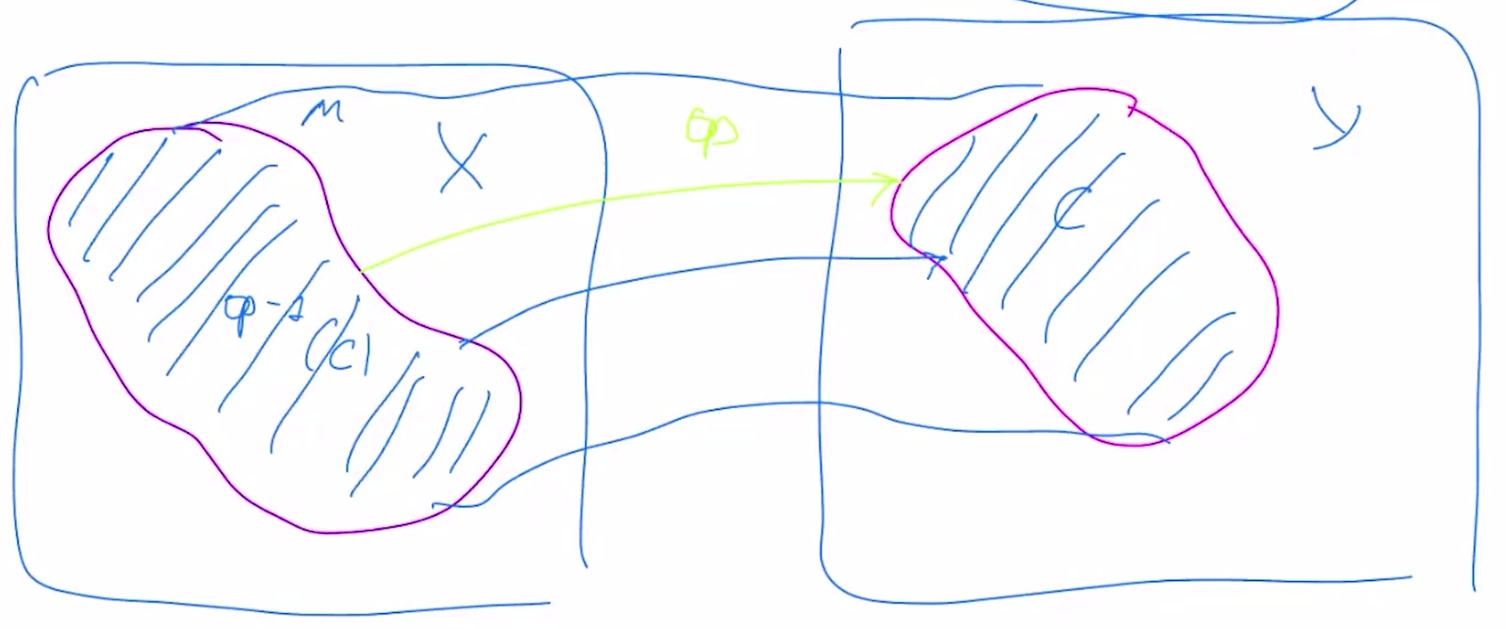
\includegraphics[width=0.99\textwidth]{images/Screenshot_14.png} 
\end{minipage}%
\hfill%


    
    push-forward меры действительно является мерой: \[ \Phi_{\#\mu}\biggl(\bigsqcup\limits_{j = 1}^\infty C_j\biggr) = \mu\biggl(\Phi^{-1}\biggl(\bigsqcup\limits_{i = 1}^\infty C_i\biggr)\biggr) = \mu\biggl(\bigsqcup\limits_{i = 1}^\infty \Phi^{-1}(C_i)\biggr) = \sum\limits_{i = 1}^\infty \mu(\Phi^{-1}(C_i)) = \sum\limits_{i = 1}^\infty \Phi_{\#\mu}(C_i)\]
\end{definition}
\begin{definition}
    Пусть есть $(X, \MM, \mu)$ и дано измеримое $\omega: X \rightarrow [0, +\infty]$. Тогда мерой $\mu$ с весом $\omega$($\omega$-взвешенной мерой $\mu$) будем называть меру $\omega\mu$ т.ч. \[\omega\mu(E) = \int\limits_E \omega(x) d\mu(x
    )\]
    Взвешенную меру можно аналогичным способом толкнуть на $Y:$ \[\Phi_{\omega\mu}(C) = \omega\mu(\Phi^{-1}(C))\]
\end{definition}

\begin{interpret}
    Следующая теорема довольна абстракна. Рассмотрим ее геометрический смысл в $\R^m$:


\begin{minipage}{1.0\textwidth}% adapt widths of minipages to your needs
    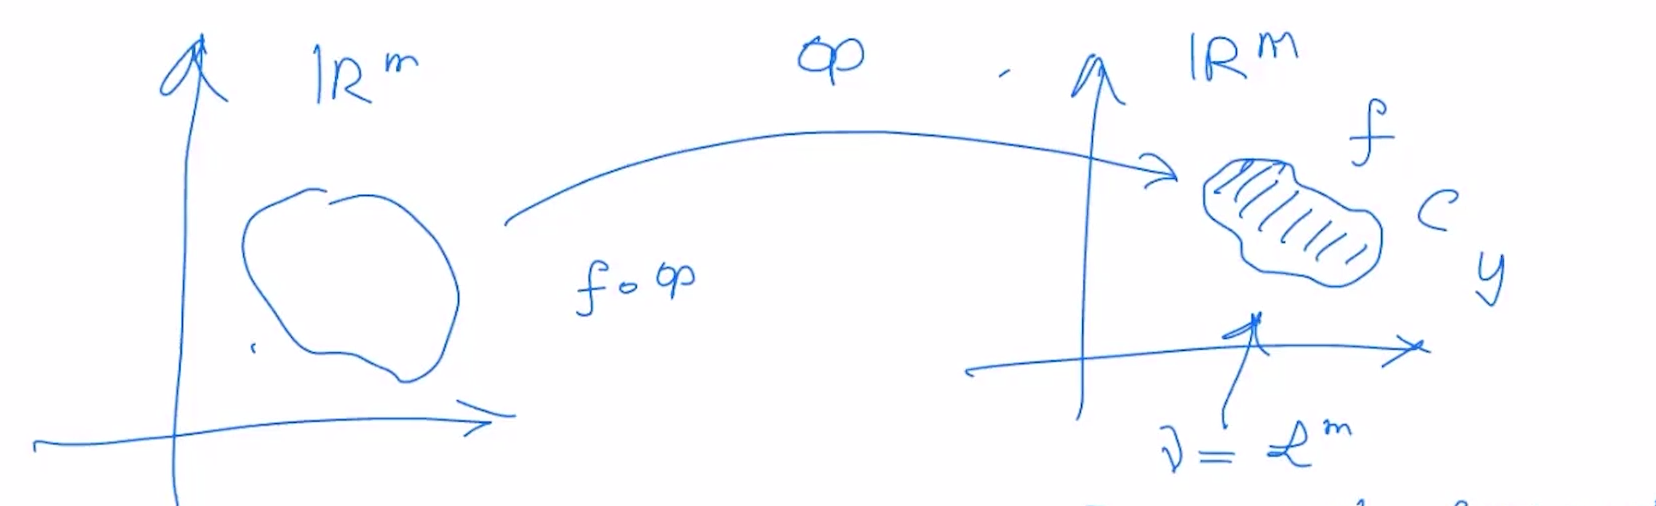
\includegraphics[width=1.0\textwidth]{images/Screenshot_15.png} 
\end{minipage}%
\hfill%
Мы хотим проинтегрировать множество $C \in Y$ по нашей классической мере в $\LL^m$ (Важно что мы сейчас в образе). Пуская мы сделали какую-то замену координат. Наше множество теперь слева. Очевидно оно как-то поменялось(например на картинке стало больше). Тогда теперь чтобы интегралы совпали нам нужно чтобы его как-то толкнуть отображением $\Phi$, но уже с весом во сколько раз изменилось множество. Этот вес равен якобиану отображения(Если отображение линейно, то доказано сверху). В общем случае идея веса в том, что локально функция представима как линейная, и поэтому вес это функция точки.
\end{interpret}

\begin{theorem}[Абстрактная замена переменной в интеграле Лебега]
    Пусть $\nu := \Phi_{\#}(\omega \mu)$, те $\nu$~---~push-forward $\omega$-взвешенной меры $\mu$ на $(Y, \NN)$. Тогда для всякой неотрицательной измеримой на $Y$ функции $f$ (или произвольной интегрируемой на $Y$) верно следующее: \[\int\limits_{Y} f(y)d\nu(y) = \int\limits_X f\circ\Phi(x)\cdot\omega(x) d\mu(x)\]
\end{theorem}
\begin{proof}
    Идея простая. Докажем для простых, а дальше используем теорему Леви. \\
    \underline{Шаг 1.} Пусть $f = \chi_C, C \in \NN$. Тогда можно заметить, что $f \circ \Phi = \chi_C \circ \Phi = \chi_{\Phi^{-1}(C)}$. И действительно: \[ f \circ \Phi(x) = \begin{cases}
        1, & \Phi(x) \in C \\ 0, & \Phi(x) \notin C 
    \end{cases} \Longrightarrow f \circ \Phi(x) = \begin{cases}
        1, & x \in \Phi^{-1}(C) \\ 0, & x \notin \Phi^{-1}(C)
    \end{cases} \Longrightarrow f \circ \Phi = \chi_{\Phi^{-1}(C)}\]
    Тогда равенство принимает вид: \[\int\limits_Y \chi_C(y)d\nu(y) = \nu(C) = \Phi_{\#\omega\mu}(C) = \omega\mu(\Phi^{-1}(C)) = \int\limits_{\Phi^{-1}(C)} \omega(x) d\mu =\int\limits_X \chi_{\Phi^{-1}(C)}(x)\cdot\omega(x) d\mu\]
    \underline{Шаг 2.}В силу линейности интеграла и аддитивности меры данное утверждение очевидным образом продолжается на произвольные неотрицательные простые функции. \\
    \underline{Шаг 3.}В общем случае, для произвольной неотрицательной измеримой $f$ мы можем рассмотреть неубывающую последовательность неотрицательных простых $f_n \rightarrow f, n \rightarrow +\infty$. Ввиду справедливости \[\int\limits_Y f_nd\nu = \int\limits_X f_n \circ \Phi \cdot \omega d\mu\]
    для всякого $n$ то переходя к пределу и используя теорему Леви мы получаем \[\int\limits_Y fd\nu = \lim\limits_{n \rightarrow +\infty} \int\limits_Y f_nd\nu = \lim\limits_{n \rightarrow +\infty} \int\limits_X f_n \circ \Phi \cdot \omega d\mu = \int\limits_X f \circ \Phi \cdot \omega d\mu\]
    Для случая интегрируемой функции $f$ мы можем заметить, что $f \circ \Phi \cdot \omega$ тоже интегрируема, и, далее пишем равенства для $f_+$ и $f_-$, вычитаем, и получаем требуемое.
\end{proof}
\begin{definition}
    Пусть $(X, \MM)$~---~измеримое пространство и $\mu, \nu$~---~2 меры на $\MM$. Будем говорить, что $\nu$ имеет плотность $\omega$ относительно $\mu$, если есть неотрицательная измеримая $\omega: X \rightarrow [0, +\infty]$ т.ч. $\nu = \omega\mu$. Иногда обозначается $\frac{d \nu}{d \nu}(x) = \omega(x)$
\end{definition}
\begin{theorem}[Критерий плотности, б/д]
    Пусть $\mu, \nu$~---~2 меры на $\sigma$-алгебре $\MM$ измеримого пространства $(X, \MM)$, а $\mu$~---~измеримая неотрицательная функция на $X$. Тогда следующие утверждения эквивалентны: \begin{itemize}
        \item $\nu$ имеет плотность $\omega$ относительно $\mu$
        \item $\forall A \in \MM \hookrightarrow \mu(A)\inf\limits_{x \in A} \omega \leq \nu(A) \leq \mu(A)\sup\limits_{x \in A} \omega$
    \end{itemize}
\end{theorem}
\begin{proof}
    (Из Макарова-Подкорытова) Необходимость очевидна. Покажем достаточность. Очевидно, что мы можем считать, что $\omega > 0$ на рассматриваем множестве $B$, поскольку \[\nu(B(\omega = 0)) = \int\limits_{B(\omega = 0)} \omega d\mu\]
    Пусть есть некоторое $q \in (0, 1)$. Рассмотрим \[B_j = \{x \in B \mid q^j \leq \omega(x) < q^{j - 1}\}, j \in \Z\]
    Такие множества образуют разбиение множества $B$, и \[\mu(B_j)q^j \leq \nu(B_j) \leq \mu(B_j)q^{j - 1}\]
    Из монотонности интеграла следует справедливость подобной оценки для $\omega$: \[\mu(B_j)q^j \leq \int\limits_{B_j}\omega d\mu \leq \mu(B_j)q^{j - 1}\]
    Суммируя по $\Z$ мы получаем следующее: \[q\int\limits_{B} \omega d\mu \leq \sum\limits_{j \in \Z} q^j\mu(B_j) \leq \nu(B) \leq \dfrac{1}{q} \sum\limits_{j \in \Z} q^j \mu(B_j) \leq \dfrac{1}{q}\int\limits_B \omega d\mu\]
    Теперь, переходя к пределу при $q \rightarrow 1$ получаем равенство.
\end{proof}
\subsection{Конкретная замена переменной в интеграле Лебега}
\begin{reminder}
    Пусть $U \subset \R^n, V \subset \R^m$~---~ открытые множества. Будем говорить, что $U$ и $V$ диффеоморфны, если существует диффеоморфизм $F$: $U \mapsto V$, то есть $F$~---~взаимооднозначное отображение $U$ на $V$, такое что $F \in C^1(U, V)$ и  $F^{-1} \in C^1(V, U)$. Если требовать именно непрерывную дифференцируемость, то такой диффеоморфизм называется гладким
\end{reminder}
Будем считать фиксированными открытые множества $G, G' \subset \R^m$ и некоторое отображение $\Phi \in C^1(G, G')$, являющееся диффеоморфизмом $G$ на $G'$.
\begin{theorem}
    Для всякого измеримого $E \subset G$ справедливо следующее равенство: \[\Phi_\#\LL^m(E) = \LL^m(\Phi(E)) = \int\limits_E|\det \D\Phi(x)|dx\]
\end{theorem}
\begin{proof}
    Напомним, что $J_\Phi = \det \D\Phi$~---~якобиан отображения $\Phi$.
    С учётом критерия достаточно доказать, что для всякого измеримого $A$ выполнено следующее неравенство: \[\LL^m(A)\inf\limits_A |J_\Phi| \leq \Phi_{\#}\LL^m(A) \leq \LL^m(A)\sup\limits_A |J_\Phi|\]
    Заметим, что достаточно доказать только правую часть неравенства, поскольку $\Phi$~---~диффеоморфизм, а значит, применяя полученное неравенство к отображению $\Phi^{-1}$ и множеству $\Phi(A)$ мы получим левую часть неравенства. $J_\Phi(x) \cdot J_{\Phi^-1}(\Phi(x)) = 1$\\
    Докажем неравенство для кубической ячейки $Q$ т.ч. $\overline{Q} \subset G$: \[\Phi_\#\LL^m(Q) \leq \sup\limits_{x \in Q} |J_\Phi|\cdot \LL^m(Q)\]
    Предположим, что существует такой куб, для которого неравенство неверно и \[\sup\limits_{x \in Q} |J_\Phi|\cdot \LL^m(Q) < \Phi_\#\LL^m(Q)\]
    В силу строгости неравенства мы можем чуть-чуть увеличить левую часть:  т.ч. \[\exists C\text{ такой что }C > \sup\limits_{x \in Q} |J_\Phi| \text{ и } C\LL^m(Q) < \Phi_\#\LL^m(Q)\]
    Разобьём каждую сторону $Q$ пополам. Те на $2^m$ равных кубических частей. По принципу Дирихле хотя бы для одной части $Q_1$ из них подобное неравенство тоже должно выполняться: \[C\LL^m(Q_1) < \Phi_\#\LL^m(Q_1)\]
    Повторяя это построение для $Q_1$, построим такую последовательность вложенных кубических ячеек \[G \supset \overline{Q} \supset \overline{Q_1} \supset \ldots \supset \overline{Q_n} \supset \ldots\]
    что \[C\LL^m(Q_n) < \Phi_\#\LL^m(Q_n)\]
    По теореме Кантора $\exists a \in \bigcap\limits_{n \in \N} \overline{Q_n}$. Пусть $L = D_a\Phi$ ~---~ линейное и обратимое отображение. Поскольку по условию $\Phi$~---~диффеоморфизм, $L$~---~обратимо, и так как $a \in \overline{Q}$, то $|\det L| = |J_\Phi(a)| < C$. Рассмотрим вспомогательное отображение которое линейно приближает окрестность точки $a$: \[\Psi(x) = a + L^{-1}(\Phi(x) - \Phi(a))\]
    Около точки $a$ отображение стремится к тождественному: \[\Psi(x) = x + o(x - a), x \rightarrow a\]
    Поэтому $\forall \epsilon > 0 \  \exists $ такой малый шар $B_{\delta(\epsilon)}(a)$, центрированный в $a$, что \[\forall x \in B \hookrightarrow \|\Psi(x) - x\| \leq \dfrac{\epsilon}{\sqrt{m}}\|x - a\| \]
    По построению $a \in \overline{Q_n}$ для всякого $n$ и $\overline{Q_n} \subset B$ для достаточно больших $n$. Тогда поскольку $\|x - a\| \leq \sqrt{m}h$ (где $h$~---~длина ребра куба $Q_n, x \in Q_n$), то $\|\Psi(x) - x\| \leq \epsilon h$ и аналогичное верно для всех координат разности $\Psi(x) - x$ а значит $\Psi(x)$ принадлежит кубу с длиной ребра $\leq(1 + 2\epsilon)h$. Тогда: \[\LL^m(\Psi(Q_n)) \leq \LL^m((1 + 2\epsilon)Q_n) \leq (1 + 2\epsilon)^mh^m = (1 + 2\epsilon)^m\LL^m(Q_n)\]
    C другой стороны, \[\LL^m(\Psi(Q_n)) = \LL^m(a + L^{-1}(\Phi(Q_n) - \Phi(a))) = \LL^m(L^{-1}\circ\Phi(Q_n)) = |\det L^{-1}| \LL^m(\Phi(Q_n))\]
    Тогда собирая все полученные неравенства, мы получаем: \[|\det L^{-1}|\LL^m(\Phi(Q_n)) \leq (1 + 2\epsilon)^m \LL^m(Q_n)\]
    Т.е. \[\Phi_\#\LL^m(Q_n) \leq (1 + 2\epsilon)^m|J_\Phi(a)|\LL^m(Q_n)\]
    Но $C\LL^m(Q_n) < \Phi_{\#}\LL^m(Q_n)$, а значит \[C \leq (1 + 2\epsilon)^m|J_\Phi(a)|\]
    Тогда возьмём $\inf$ по всем $\epsilon$, и получим $C \leq |J_\Phi(a)|$. Но $C > \sup\limits_{x \in Q} |J_\Phi|$, а поскольку $a \in Q$ то мы получаем противоречие, и неравенство $\Phi_\#\LL^m(Q) \leq \LL(Q)\sup\limits_{x \in Q} |J_\Phi|$ выполняется для всех кубических ячеек $Q$: их замыкание лежит в $G$. Но любое открытое множество представляется как дизъюнктивное объединение счётного числа кубических ячеек, а значит неравенство верно и для них. Теперь, используя регулярность меры Лебега, мы можем обобщить результат на произвольное измеримое множество $A$: \[\Phi_\#\LL^m(A) \leq \inf\limits_{A \subset \Omega \subset G} \Phi_\#\LL^m(\Omega) \leq \inf\limits_{A \subset \Omega \subset G} \LL^m(\Omega) \sup\limits_\Omega |J_\Phi| \leq \LL^m(A) \cdot \sup\limits_A |J_\Phi|\]
\end{proof}
\begin{corollary}
    Из непрерывности $|J_\Phi|$ и предыдущей теоремы следует, что \[|J_\Phi(a)| = \lim\limits_{A \rightarrow a} \dfrac{\LL^m(\Phi(A))}{\LL^m(A)}\]
    Где под пределом мы понимаем $\forall \epsilon > 0 \exists \delta > 0 \forall A \in \MM^m \wedge A \subset B_\delta(a) \wedge \LL^m(A) > 0 \hookrightarrow |\frac{\LL^m(\Phi(A))}{\LL^m(A)} - |J_\Phi(a)|| < \epsilon$.
\end{corollary}
\begin{theorem}
    Пусть $\Phi$~---~диффеоморфизм $G$ на $G'$. Тогда для любой измеримой неотрицательной функции $f$ на $G'$ верно следующее: \[\int\limits_{G'} fdy = \int\limits_G f \circ \Phi \cdot |J_\Phi|dx\]
\end{theorem}
\begin{proof}
    Результат очевиден в силу предыдущей теоремы и теоремы об абстрактной замене переменных в интеграле Лебега при подстановке \[\mu = \LL^m, \nu = \LL^m, \omega = |J_\Phi|, X = G, Y = G'\]
\end{proof}